\chapter{Probabilistic Trajectory Prediction}
\label{chap:2}
%
This chapter introduces a concept and theoretical framework for all steps which are necessary to solve the problem of motion recognition and prediction with our proposed probabilistic intention prediction algorithm. 

\section{Including Prior Information To Algorithm}

For testing the probabilistic intention prediction algorithm we have two environment setups: X and T intersection, Figure~\ref{fig:XandT}. Information about the map is crucial because it gives the value of initial belief ($b_{0}$), one of the most important variables of our initial probabilistic model at the beginning of prediction-making. 

\begin{figure}[H]
	\centering  	
	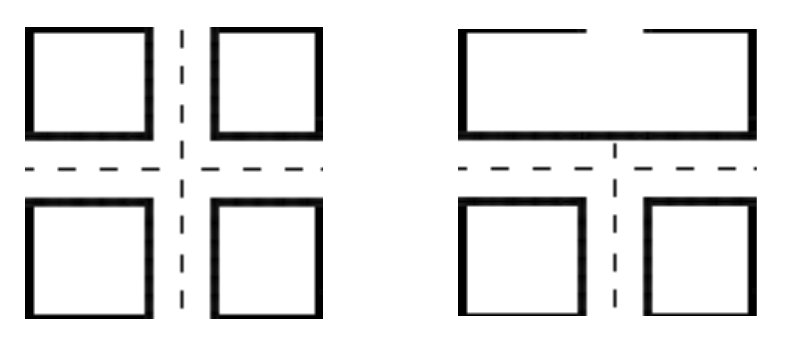
\includegraphics[width=8cm]{img/XandT.png}
	\caption{X intersection map in the left and T intersection map on the right}
	\label{fig:XandT}    
\end{figure}

In the map with X intersection, we assume that the probability to go to any direction is equal, so initial belief value is $b_0 \text{[right, straight, left]} = (0.333, 0.333, 0.333)$. In the case of T intersection from the very beginning, we know that one direction is not available - the car can go only straight or right. Considering this information we need to recalculate the value of initial belief since it can't be equal anymore. Initial belief on T intersection is calculated using information about number of demonstrations we used for algorithm learning probabilistic prediction model. We calculate initial belief for right and left directions using these formulas:
\begin{equation}
b_{0}(right) = \frac{R}{L + R}, b_{0}(left) = \frac{L}{L + R},
\end{equation}
where R and L stand for trajectories going to the right and left in our predefined \gls{DB}.
To be able to define initial belief, the first step of intention prediction algorithm is to recognize the map. There were two map recognition methods tested in the algorithm. Results proved that both methods for map recognition are working, but the first method is a very simple one and used only contours in the map, which means that is a map will have slight changes like new obstacles, new code adaptation would be needed with this method. Due to this reason another map recognition program was created which uses \gls{SSIM} and recognize map according to some common similarities - all description is in the previous chapter. \\
Subsections below will give an explanation of two different methods, both were using \gls{OpenCV} library for Python, we used for map recognition. \gls{OpenCV} - is an open source library for computer vision and machine learning programs. It was developed to grant a common infrastructure for computer vision applications and to speed up the usage of machine apprehension \cite{aboutOpenCV}. 

\subsection{Map Recognition using Contours}

Map recognition using contours in OpenCV library is a relatively simple method, but a helpful tool for object recognition (as well as, for object detection or/and shape analysis), using the number of counters in the pictures and according to it, making recognition. \\
First of all, let's answer the question, what are contours? We can define contours as a curve which joins all continuous points, which has the same colour or the same intensity. The tool works in this way, that before contours detection it applies threshold (as in our case) or canny edge filter. Contours in OpenCV works in greyscale and to have the best results object of interest should be white in black background (or vice versus) \cite{contours}. 
Let's use the code snippet to explain contours better:
\begin{lstlisting}
import numpy as np
import cv2

img1 = cv2.imread('maps/testmap.png')
gray1 = cv2.cvtColor(img1, cv2.COLOR_BGR2GRAY)
ret1, thresh1 = cv2.threshold(gray1, 127, 255, 1)
contours1, h1 = cv2.findContours(thresh1, 1, 2)
\end{lstlisting}

In cv2.findContours() function there are $3$ arguments: first of them is source image, converted to greyscale. The second one is contour retrieval mode (we assigned it to be 1 since we are interested to retrieve contours only, not to create any hierarchy/parent-child level). The last argument means contour approximation method. Contour approximation modified a contour shape to another shape with fewer peaks depending on the accuracy we choose (using Douglas-Peucker algorithm \cite{aprox}). \\
To understand this, let's use another snippet of code:
\begin{lstlisting}
approx1 = cv2.approxPolyDP(cnt1, 0.01 * cv2.arcLength(cnt1, True), True)
\end{lstlisting}
Without function which approximate shape we usually are not getting the correct form, due to some "visual information noises" or due to other problems in the source image. Using shape approximate function we use maximum distance from contour to approximated contour - this is a parameter of precision. This parameter is the second argument in approxPolyDP() function ("0.01 * cv2.arcLength(cnt1, True)"). To chose this parameter correctly is important because due to it we receive the good or bad result of finding the contour method.\\
To see the output of the method we can draw contours, using cv.drawContours function (code snippet below):
\begin{lstlisting}
cv2.drawContours(img1, [cnt1], 0, (0, 0, 255), -1)
\end{lstlisting}
The first argument of the function is the source image, the second argument are contours which were found, the third argument is counter index and the last argument is colour. The Figure~\ref{fig:count} shows how the output of function looks like.

\begin{figure}[H]
	\centering  	
	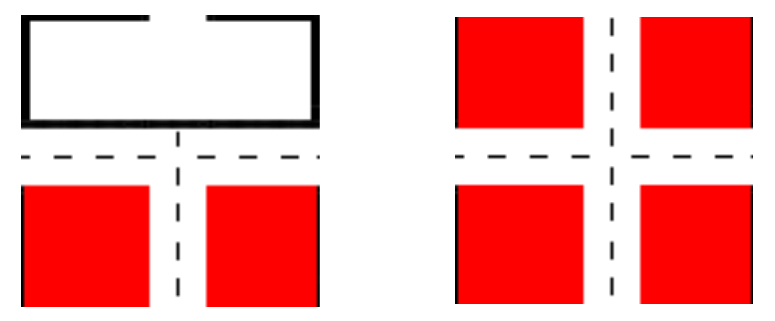
\includegraphics[width=8cm]{img/countours.png}
	\caption{Contours for T (left) and for X (right) intersection maps, received as one of outputs of map recognition, using contours method}
	\label{fig:count}    
\end{figure}

Having this information map is recognized by a number of contours it has in the image source (T intersection has $4$ contours and X intersection has $8$). As mentioned before this method is relatively simple to use, but it will cause problems in map recognition if there will be more contours inside of the image of the map (i.e. if there will be some obstacles depicted on the map T intersection) and it will cause problems in recognition. Due to this reason another map recognition method was proposed.

\subsection{Map Recognition using \gls{SSIM}}

For humans, it is quite easy to find differences between images, we are quick to recognize what is missing in one or another image - we are good at noticing how much one image similar to another. The first method we described for map recognition cannot tell how much images differs between each other but for better map recognition we need to be able to recognize similar forms in the picture (e.g. we should be able to recognize T intersection even if one image of T intersection has obstacles on the road or trees, houses on the side, etc.). For another type of map recognition, we proposed to use \gls{SSIM}. \gls{SSIM} is a method for estimating similarities between two images. The \gls{SSIM} index can be described as a measure of quality for one image after comparing with another. Mode details on \gls{SSIM} can be found in \cite{SSIM}.\\
To be able to work with \gls{SSIM} at first we need to have any size \gls{DB} of images of the same object (set of X and T intersection images). Figure~\ref{fig:db} show dataset for testing images similarities for T intersection. 

\begin{figure}[H]
	\centering  	
	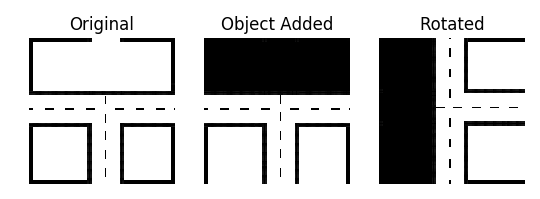
\includegraphics[width=10cm]{img/DB.png}
	\caption{Dataset for T intersection recognition, used for testing \gls{SSIM} method}
	\label{fig:db}    
\end{figure}

For image similarity \gls{SSIM} method calculates a Structural Similarity Index by the formula below:

\begin{equation}
\begin{split}
SSIM(x,y) = \displaystyle \frac{(2I_{x}I_{y} + Cont_{1})(2SCont_{xy} + Cont_{2})}{(I_{x}^2 + I_{y}^2 + Cont_{1})(SCont_{x}^2 + SCont_{y}^2 + Cont_{2})}
\end{split}
\label{eqn:SSI}
\end{equation}
where Cont is contrast and I and SCont are estimated intensity and estimated signal contrast respectively. \\
\gls{SSIM} tries to model the comprehended difference in the structure of the image. During calculation of the structural similarity index, two windows (i.e. small sub-samples) are compared. This allows us to reach robust approach that is able to see changes in the image structure, rather than just the perceived change. Structural similarity index formula considers position (x and y values) of the N x N window in each image, the mean of the pixel intensities and the variance of intensities in both directions, along with the covariance values \cite{SSIMII}. Figure~\ref{fig:res} shows structural similarity index value for different images from data set as compared with original one.

\begin{figure}[H]
	\centering  	
	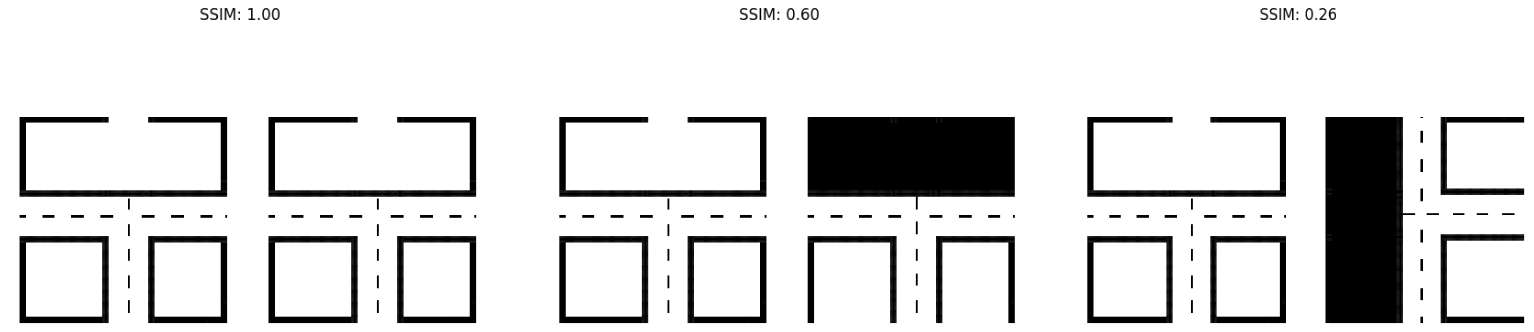
\includegraphics[width=14cm]{img/results.png}
	\caption{\gls{SSIM} value for different images from data set as compared with the original one. Index of similarity for the original picture is equal to 1, for pictures with added object similarity index is equal to 0.6 and index of similarity for a rotated picture with object added is 0.26. SSIM index can vary from -1 to 1}
	\label{fig:res}    
\end{figure}

\gls{SSIM} value is between $-1$ and $1$, where $-1$ shows no similarity and $1$ shows perfect matching. We can choose the level is similarity (value of structural similarity index) is good for our recognition.

\section{Trajectory Preprocessing}

Our \gls{DB} has a various number of demonstrations of different movement classes, which we used for teaching algorithm initial probabilistic prediction model. Since all trajectories are different movement wise, they are not equal by length (i.e. one trajectory might have $8,000$ time steps, another one $7,600$, third $9,621$, etc.). This happened because of the different pace of car while recording data, different movements, like turning, which can reduce or improve the length of the trajectory. This is a problem for probabilistic intention prediction algorithm. Having different lengths trajectories makes some problems in further calculations, comparison of results, the calculation over thousands of steps also has a longer computation time, etc. Because of that, trajectories unification is necessary (at least with trajectories we already have recorded, for trajectories which are getting in real time additional step is necessary and it is described at the end of this chapter).   \\
Trajectories unification was done using interpolation when all trajectories transformed to have an equal number of time steps (chosen by us), in spite of the fact that original number of time steps are unequal. In mathematics interpolation is a method of building new data points inside the range of a discrete set of known/given data points. \\
If we consider that we have point A and point B with coordinates ($x_{A}, y_{A}$) and ($x_{B}, y_{B}$), formula for finding values for interpolated point with coordinates ($x_{int.}, y_{int.}$), can be calculated using formula below:

\begin{equation}
\begin{split}
y_{int.} = \displaystyle y_{A} + (y_{B} - y_{A}) \frac {x_{int.} - x_{A}}{x_{B} - x_{A}} 
\end{split}
\label{eqn:interpolated}
\end{equation}


The pseudo code below (Figure~\ref{fig:pseudoInter}) shows the way of interpolation in this project.

\begin{figure}[H]
	\centering  	
	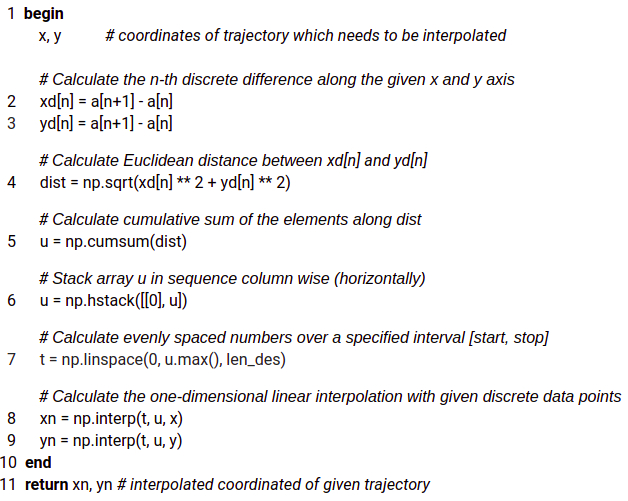
\includegraphics[width=13cm]{img/interpolation.jpg}
	\caption{Pseudo code for interpolation process}
	\label{fig:pseudoInter}    
\end{figure}

Figure~\ref{fig:InterExam} illustrates $3$ original trajectories for each movement class in red and $3$ interpolated version of the same trajectories in blue. Original trajectory, which goes to the right has $7,581$ time steps, while straight trajectory has $13,666$ and the left trajectory has $10,929$ time steps after interpolation all trajectories contain 10 steps.

\begin{figure}[H]
	\centering  	
	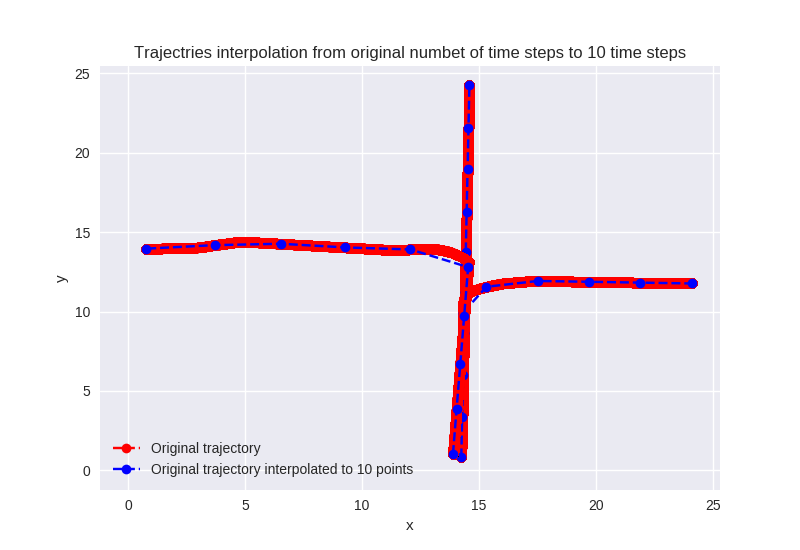
\includegraphics[width=10cm]{img/trajInnter.png}
	\caption{Original and Interpolated Trajectories. Red lines show the original trajectories of going to the right, left and straight direction. The number of time steps which has original trajectories which go to the right, straight and left have $7,581$, $13,666$ and $10,929$ time steps respectively. Blue dotted line represents interpolation of the same trajectories. Interpolation was done for $10$ time steps}
	\label{fig:InterExam}    
\end{figure}

As can be seen, interpolation does not distort trajectories and can be used in further calculations.\\
After all trajectory unification is done, mean of trajectories and variance per each time steps need to be found. More information how to do this is in this chapter below. \\
After we include unification process for demonstrations into our algorithm, learning of probabilistic model begins.

\section{Learning Probabilistic Trajectory Models From Demonstrations}

Our proposed probabilistic intention prediction algorithm learning from the set of previously recorded demonstrations. More about how data was collected is written in Chapter 4. Every trajectory can be considered as a generic vector, consisting of all values learned that the time period and we also have a vector of all coordinates, which was recorded at a particular time step \textit{t}. Trajectories can be mono-dimensional or multidimensional, in our case we are working with two-dimensional space, having x and y coordinates. We want to note that due to different trajectories, the length of each trajectory is not the same. To find a common representation for learning purposes, we needed to have the same length for all trajectories. We applied interpolation to achieved that (more details in this Chapter, just above). \\
To check every trajectory in \gls{DB} is computationally difficult, takes much more time to process and give not so much movement freedom while testing algorithm. To avoid that the mean trajectory and covariance matrix for each movement class, using formulas~\ref{eqn:meanXY}, ~\ref{eqn:COV}:

\begin{equation}
\begin{split}
\mu_x = \displaystyle \frac{\sum_{i=1}^{n} x_i}{n},     \mu_y = \displaystyle \frac{\sum_{i=1}^{n} y_i}{n}
\end{split}
\label{eqn:meanXY}
\end{equation}

\begin{equation}
\begin{split}
\bm{\Sigma{x}} = \displaystyle \frac{\sum_{i=1}^{n} (x_i - \mu_{x}) (x_i - \mu_{x})^T}{n-1}, \bm{\Sigma{y}} = \displaystyle \frac{\sum_{i=1}^{n} (y_i - \mu_{y}) (y_i - \mu_{y})^T}{n-1},  
\end{split}
\label{eqn:COV}
\end{equation}

where $x_i \text{and} y_i$, x and y values from all trajectories at time step \textit{t}, n is number of trajectories, $\mu{x}$ and  $\mu{y}$ are mean values of x and y from all trajectories at time step, $\Sigma{x}$ and $\Sigma{y}$ covariance matrix.


The proposed algorithm uses the distribution over the observed trajectories. To recognize movement class, we use the movement that passes by the mean of the distribution. \\
When we covered all this and we have probabilistic prediction model learned we can go into an explanation of probabilistic estimation methods.

\section{Probabilistic Estimation Methods for Movement and Intention Prediction}

Reasonable prediction and following decision-making process require considering uncertainty and objectives for the current situation. In this section, uncertainty will be represented as a probability distribution. \\
Uncertainty can be a result of partial information about the state of the world. In a real world trying to fulfill any given task, it is possible to meet various reasons which do not allow to finish a task without any difficulties. This means, that with information we have at hand, it is hardly possible to make a task evaluation with complete certainty. \\
Uncertainty can appear from practical and theoretical limitations while trying to predict future events, e.g., trying to exactly predict how a human would react in one situation or another, a decision support system would need to consider a model of the human brain. Even if the operation is known very well, it is still difficult to predict the end state and next actions which will be taken, due to spontaneous failures or other agent actions. \\
A robust prediction (and later decision) making system need to take into account sources of uncertainty, which exist in the current state and consider it when computing the future outcomes for events. In order to describe uncertainty
computationally, it needs to have a formal representation. 

\subsection{Belief State and Probability}

Solving tasks which involve uncertainty, it is very important to be able to compare the credibility of different statements. For example, if belief for action E is stronger than our belief for action T, then E $\succ$ T. If E and T have the same degree of belief, then E $\sim$ T. \\
It is also beneficial to be able to compare beliefs about statements considering some given information, e.g., we can say that likelihood that action C may happen while E condition is happening is bigger than having T, then this expression would be written (E | C ) $\succ$ (T | C ). \\
In order to make particular assumptions about the relationships of the operators $\succ$, $\prec$ and $\sim$. The assumption of \textit{universal comparability} and \textit{transitivity} assumptions requires to hold the same mathematical rules. Both assumptions allow representing degrees of belief by a real-valued function \cite{BOOK}, i.e. probability function P can be expressed like that:
\[ P(A|C) > P(B|C) \iff (A|C) \succ (B|C) \]
\[P(A|C) = P(B|C) \iff (A|C) \sim (B|C), \]
where $P(A|C)$ and $P(B|C)$ are conditional probabilities, with A, B and C events. $P(A|C)$ can be read as "the conditional probability that even A will happened given some event C". If new assumptions about the probability P form, then P need to satisfy the main axioms of probability: 0 $\leqslant$ P (A | B ) $\leqslant$ 1. If we are sure that A action will happen when B action is given then P (A | B ) = 1. If A action will not happen when B action is given, then
P (A | B ) = 0. \\
Deep review about probability theory won't be provided in here, but this work relies on important probabilities properties. The first of them is a definition of \textit{conditional probability}:

\begin{equation}
P(A|B)=\frac{P(A,B)}{P(B)},
\end{equation}

where P(A, B) shows the probability of A and B both being true. \\
Another property which is important is the \textit{law of total probability}, which states that if $\beta$ is a set of "mutually exclusive and exhaustive propositions" \cite{BOOK}, then

\begin{equation}
P(A|C)=\displaystyle \sum_{B \epsilon \beta}{P(A|B,C)P(B|C)}
\end{equation}

Finally, the most important rule for further work comes from the definition of \textit{conditional probability}:

\begin{equation}
P(A|B)=\frac{P(B|A)P(A)}{P(B)}.
\end{equation}

This equation is known as \textbf{\textit{Bayes’ rule}}, where $P(A|B)$ is \textbf{posterior}, in other words, it is something we are trying to evaluate, $P(B|A)$ is is \text{likelihood}, it is the probability of observing the proofs, given having an initial hypothesis, $P(A)$ is a \textbf{prior}, it is the probability of hypothesis without any additional information from before and $P(B)$ is a \textbf{marginal likelihood}, it is the complete probability of observing evidence for our hypothesis. This formula will be very important for the following work. \\
But still, after this short introduction, question what exactly belief state is, still exists. One option to answer this would be the most believable next state for an examined object, considering experience in the past, which is given. This idea can be sound basis for predictions in some cases, but in general, this idea is not sufficient. Being able to operate efficiently the degree of uncertainty must be taken into account, e.g. if the main agent is confused what future state could be, it could be good to ask directions, take a look into the map, search for reference point, etc. \\
Other options for belief computation would be using probability distributions over states of the world, which we have. In this case, distributions encode the subjective probability for the main agent and include information about the state of the world and give a basis for taking action under uncertainty we have.  Moreover, sufficient statistical information of action made in the past and initial belief state of the agent is comprised, i.e. computed belief state for the current agent’s state and additional information about its past observations and/or action made, would provide any further information about the current state of the world \cite{belief}. \\
\textbf{Computing belief states}\cite{belief}: \\
A belief \textit{b} is a probability distribution over state space $\mathscr{S}$, \textit{b(s)} is the probability set to world state \textit{s} by belief state \textit{b}. The axioms for belief state is the same as for probabilities: 0 $\leqslant$ b(s) $\leqslant$ 1, for all s $\epsilon$ $\mathscr{S}$ and $\sum_{s \epsilon \mathscr{S} } b(s) = 1.$ At every new step, new belief \textit{b'} must be  computed given old belief \textit{b}, an action \textit{a} and an observation \textit{o}. The new belief of an new state \textit{b'(s')} can be calculated using formula:

\begin{equation}
\begin{split}
b'(s') = & \displaystyle Pr(s'|o, a, b) \\ 
& = \displaystyle \frac{Pr(o|s', a, b) Pr(s'|a, b)}{Pr(o|a, b)} \\
& = \displaystyle \frac{Pr(o|s', a) \sum_{s \epsilon \mathscr{S}} Pr(s'|a, b, s) Pr(s|a, b)}{Pr(o|a, b)} \\
& = \displaystyle \frac{O(s', a, o) \sum_{s \epsilon \mathscr{S}} T(s, a, s') b(s)}{Pr(o|a, b) }, 
\end{split}
\label{eqn:Dem}
\end{equation}

where the denominator of formula~\ref{eqn:Dem}, Pr(o | a, b), can be interpreted as a normalizing factor, which is independent of next state s', which causes the sum of belief of all possible next states to 1. The task of the state estimation function SE(b, a, o) is to update the belief state based on the \textit{a, o} and the previous \textit{b}, as its output gives new belief for new state \textit{b'}, $T(s, a, s')$ is a transition from one state to another probability function. \\
In later work, belief update will act an important role, but it will be computed using different components. Further detail description of belief computation related to this work will be provided.

\subsection{Modeling Belief for Prediction Making}

A Bayesian version of a Gaussian Mixture Model is used for calculating the belief each trajectory class and this section gives definitions for beliefs representing for a car over trajectory movement classes (right,straight and left). \\
Our observation is the current position of the car, which means that trajectory class is partially observable, due to that our belief is represented as a probability distribution over all trajectory classes. \\
For maintaining correct belief, updates must be done every time step. Updating belief constantly is important because sudden position change can show drivers' intentions and what his next steps could be. To be able to predict possible future movement, current position information need to consider every time when belief update is calculated. The belief update is calculated using Bayes Rule, formula~\ref{eqn:formula1}: 

\begin{equation}
\begin{split}
b_{t+1}(k) = & \displaystyle Pr(k|o_{t}, b) \\ 
& = \displaystyle \frac{Pr(o_{t}|k, b) Pr(k|b)}{Pr(o_{t}|b)} \\
& = \displaystyle \frac{Pr(o_{t}|k, b) Pr(k|b)}{ \sum_{j} Pr(o_{t}|b) Pr(j|b)} \\
& = \displaystyle \frac{Pr(o_{t}|k, b) b_{t}(k)}{ \sum_{j} Pr(o_{t}|j, b) Pr(j|b)}
\end{split}
\label{eqn:formula1}
\end{equation}

With given formula belief for future step $b_{t+1}(k)$ for a predefined class is calculated. $b_{t}(k)$ is a belief from the last calculation, denominator of function is a normalization function for the current step. $Pr(o_{t} | k, b)$ is the car position observation model, which returns the probability (or likelihood) of going to any direction from the current position, observed with $o_{t}$. This likelihood can be calculated using multivariable Gaussian probability distribution function $\mathcal{N}(x|\mu,\Sigma)$. This probability distribution function looks the following:

\begin{equation}
\begin{split}
\mathcal{N}(x|\mu,\Sigma) = \displaystyle \frac{1}{\sqrt{(2 \pi)^n det(\Sigma)}} exp(-\frac{1}{2}(x-\mu)^T\Sigma^{-1}(x-\mu)), 
\end{split}
\label{eqn:formula2}
\end{equation}

where dimensionality n = 2 and x is a currently observed position of the car $x = (o_t^x, o_t^y)^T$, $\mu$ is a mean from all predefined trajectories in \gls{DB} for the same class $\mu_k  = (\mu_{t,k}^x, \mu_{t,k}^y)^T$ and $\Sigma$ is a covariance matrix of all predefined trajectories in data base for the same class $\Sigma_k  = (\Sigma_{t,k}^x, \Sigma_{t,k}^y)^T$. Mean for x and for y coordinates and variance was found before using formulas ~\ref{eqn:meanXY} and ~\ref{eqn:COV}

The denominator of formula~\ref{eqn:formula1} is the so-called normalization factor, which sums all likelihoods of the car over all movement classes at the current time step. The final result of formula will return updated belief that car is moving towards any of classes. \\
Figure~\ref{fig:PseudoBelief} shows pseudo-code how belief updates are made over time, as an input having current belief $b_t$ at time step t, current car position $x_t, y_t$ from the last made observation, as well we have before calculated mean and covariance values at that time, $\mu_{t,k}^x, \mu_{t,k}^y$ and $\Sigma_{t,k}^x, \Sigma_{t,k}^y$ respectively.

\begin{figure}[H]
	\centering  	
	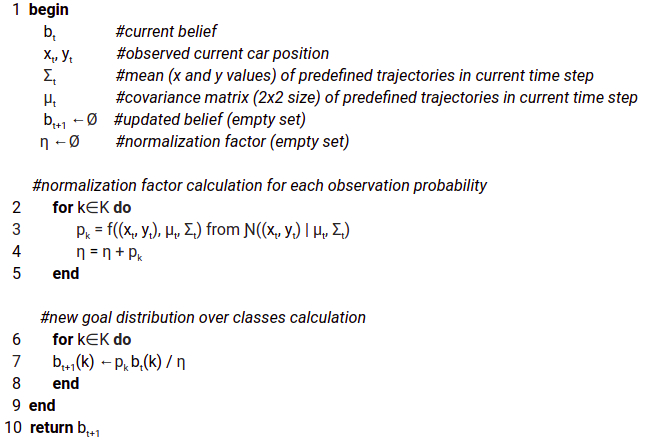
\includegraphics[width=13cm]{img/pseudoBeliefUpdate.jpg}
	\caption{Pseudo Code for Updating belief}
	\label{fig:PseudoBelief}    
\end{figure}

This cycle repeats while the car is moving and at every time step, it gives a new prediction of what future movement is going to be. Results of testing probabilistic intention prediction algorithm are given in the next chapter.

\section{Trajectory Scaling}

Computation time for prediction is one of the main things which needs to be fast. Even though more belief updates give more precise results, more computations take more time. In this project, we took various numbers of time steps and compared results to get them as precise as possible and have fewer time steps (e.g. we aimed to keep precision of trajectory of $100$-time steps but have only 10-time steps trajectory). \\
To achieve desired results, we used "toy problem" approach. \cite{ToyPr} defines it as "In scientific disciplines, a toy problem is a problem that is not of immediate scientific interest, yet is used as an expository device to illustrate a trait that may be shared by other, more complicated, instances of the problem, or as a way to explain a particular, more general, problem-solving technique". \\
We raised a likelihood (formula~\ref{eqn:formula2}) of the trajectory with a bigger number of time steps at every time step $\frac{1}{\frac{T}{t}}$ and updated formula~\ref{eqn:formula2} looks like shown below. After scaling we compared results of matching points in each trajectories. After these modifications formula~\ref{eqn:formula1}, looks like: 

\begin{equation}
\begin{split}
b_{t+1}(k) = & \displaystyle \frac{(Pr(o_{t}|k, b))^{t/T} b_{t}(k)}{ \sum_{j} (Pr(o_{t}|j, b))^{t/T} Pr(j|b)}, 
\end{split}
\label{eqn:formula5}
\end{equation}
where T and t are the bigger and the smaller numbers of times step in compared trajectories.
To simplify all this, let's have an example: let's imagine we have the trajectory interpolated to $100$-time steps and we want to see how results differ when we do belief updates all $100$ times with doing belief at every $10$th step ($10$th, $20$th, ..., $90$th, $100$th). Without doing any changes in the original code, these results are not matching, in fact, they differ quite a lot. But if we raise likelihood (formula~\ref{eqn:formula2}) of the trajectory where belief is updating $100$ times by $\frac{1}{\frac{100}{10}} = \frac{1}{10}$ at every time step and then do belief updates as normal and compare them with belief updates which are calculated every $10$th step with making no changes in the original code. After comparison of these results, it was easy to see that results are matching or are close enough to each other. The pseudo code of the given example is in Figure~\ref{fig:PseudoScalling}.

\begin{figure}[H]
	\centering  	
	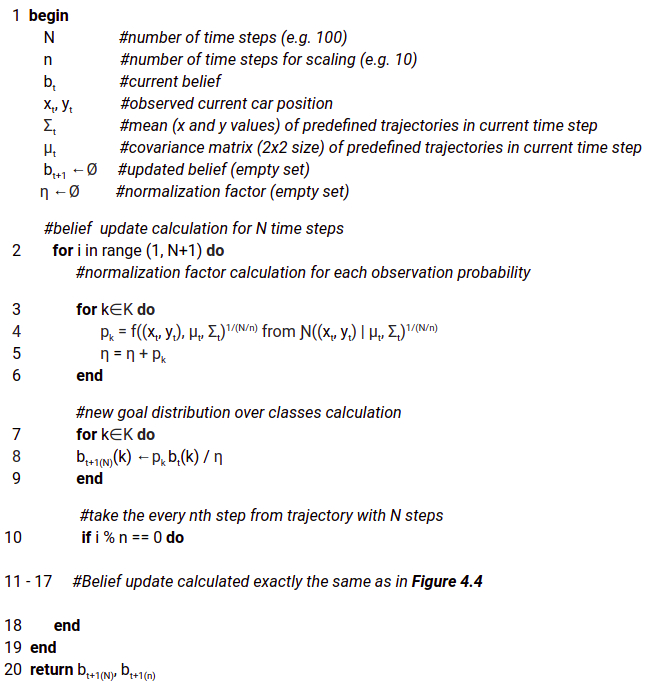
\includegraphics[width=13cm]{img/Pseudo4Scalling.jpg}
	\caption{Pseudo Code for Scaling Trajectory for Belief Update}
	\label{fig:PseudoScalling}    
\end{figure}

Having this in mind we can make our prediction making the process faster and more precise. 

\section{Making Prediction While Working With Real Time Data}

Another simulation experiment was to try to predict movement with data which is not recorded in advance. For that the same probabilistic intention prediction algorithm was used, just observations about current position came not from the trajectory which was prepared (recorded and then interpolated) for calculations in advance, but from a real-time simulation with \gls{ROS} and its visualization in \gls{RViz}, meaning that we did not have all trajectory from the beginning, which forced us to slightly change probabilistic intention prediction algorithm. When we were working with predefined testing trajectories, we treated them exactly the same as algorithm training data: we interpolated trajectory with the same amount on time steps as we did with trajectories from \gls{DB} and then for prediction making, to formula~\ref{eqn:formula1} we put the current position of the testing trajectory for the first time step, took mean trajectory position and variance value for the first time step from our \gls{DB} and so on until the trajectory is over. Due to the problem that we have no idea how many steps trajectory will have, we could not interpolate our testing trajectory and we can't treat the nth step in interpolated (dataset) trajectory with nth step from our real-time testing trajectory, because these steps can be very far away from each other and prediction results will make no sense and the other reason that interpolated trajectory will end at some point (much faster than our test drive in simulation) and then we will get an error, because there will be no interpolated values (i.e. our data set is interpolated for $10$ steps, the first $10$ steps are just beginning for testing trajectory and during $11$th step we will get an error since there is no $11$th step in interpolated data set and so on). \\
Because of that, we used the current observed position and using Euclidean distance formula~\ref{eqn:distance} to calculate the distance between the current car position and all points in the interpolated trajectory. 

\begin{equation}
\begin{split}
dist = \displaystyle \sqrt{(x - x_{int.})^2 + (y - y_{int.})^2},
\end{split}
\label{eqn:distance}
\end{equation}
where x and y are currently observed position values $x_{int.} \text{and} y_{int.}$ is values per each time step of interpolated trajectory. Having all these values calculated, the smallest distance value is selected, Having that to formula~\ref{eqn:formula1} we can put the closest value of mean trajectory and variance values for the same time step. \\
There are other existing methods, which could be adopted for find differences between testing and trajectories in \gls{DB}, such as \gls{DTW} in \cite{DTW} or \cite{PossExecution} which incorporated local variability in the execution of position.

\subsection{Probabilistic Movement Primitives (\gls{ProMPs})}

\textcolor{red}{TO FIX} 

As in previous cases, we have a set of demonstrations which are pre-recorded in advance. We can see each demonstration as vector or time-dependent variables, and each time step as a vector, containing all variables which were learned at that particular timestep \textit{t}. Our demonstrations are two-dimensional (however, they can be mono- or multi-dimensional). As in previous cases, the length of the demonstrations are not matching, due to that, we used the same time modulation for $100$-time steps as before. \\
\gls{ProMPs} uses a generic Bayesian parametric model to express demonstrations:

\begin{equation}
\begin{split}
x_{reconstructed}(t) = \displaystyle \Phi_{t}\omega,
\end{split}
\label{eqn:ProMPs}
\end{equation}

where $x(t)$ x dimension depending on time step $\omega \epsilon R^M$ is \gls{RBF} weights, not depending on time, $\Phi_{t}$ is a vector of \gls{RBF}, at time step \textit{t}, parameter meaning the number of \gls{RBF} is M. $\Phi_(t)$ is expressed as:

\begin{equation}
\begin{split}
\Phi_{t} = \displaystyle [\psi_{1}(t), \psi_{2}(t), ..., \psi_{M}(t)], 
\end{split}
\label{eqn:RBF}
\end{equation}

with
\[ 
\left \{
\begin{tabular}{ccc}
$ \psi_{i}(t) = \frac{-(t - c(i))^2}{2h} $ \\
$ c(i) = i/M $ \\
$ h = 1/M^2 $ 
\end{tabular}
\right \}
\] 
where M denotes the number of \gls{RBF}, h denotes standard deviation and c denotes mean.
For each demonstration we compute one weight parameter vector $\omega_{i}$, to have expression of formula~\ref{eqn:RBF} for each \gls{RBF}. Weights for each \gls{RBF} are computed using, Least Mean Square algorithm, together with added diagonal term (in case matrices in Least Mean Square algorithm are not invertible). $\omega_{i}$ for x dimension is calculated using:

\begin{equation}
\begin{split}
\omega_{i} = \displaystyle (\Phi_{t}^T \Phi_{t} + \lambda)^{-1} \Phi_{t}^T,  x_{i}(t), 
\end{split}
\label{eqn:RBF}
\end{equation}
where $\lambda)$ is a diagonal term, the smallest singular value of matrix $\Phi_{t}^T \Phi_{t}$. 
Once we obtain all values for $\omega = {\omega_{1}, .... , \omega_{n}}$, we calculate Normal distributions:

\begin{equation}
\begin{split}
p(\omega) = \displaystyle \mathcal{N}(\mu_{\omega}, \sum{\omega}), 
\end{split}
\label{eqn:123}
\end{equation}

with
\begin{equation}
\begin{split}
\mu_{\omega} = \displaystyle \frac{\sum_{i=1}^{n}\omega_{i}}{n},  \sum{\omega} = \displaystyle \frac{\sum_{i=1}^{n} (\omega_{i} - \mu_{\omega})^T (\omega_{i} - \mu_{\omega}) }{n-1},
\end{split}
\label{eqn:01}
\end{equation}
 
where $\mu_{\omega}$ is a mean if weights and $\sum_{\omega}$ is covariance.
Having the distribution over demonstrations it is possible to represent movement primitives which pass through the mean value. This representation can be found in Chapter 5, Section 5.1.4. \\
But before representing trajectory with leaned movement primitives, it is very important to choose the right number for \glspl{RBF}. To few functions can lead us to insufficiency of trajectories approximation, while too many can cause over-fitting problems. We chose the right number for \glspl{RBF} by computing root mean square deviation, which can be computed as follows:

\begin{equation}
\begin{split}
\epsilon = \frac{\sum_{n}(\xi - \xi_{reconst})^2}{N}, 
\end{split}
\label{eqn:1234}
\end{equation}
where $\epsilon$ is error for trajectory, N - number of trajectories, $\xi$ - original trajectory and $\xi_{reconst}$ - reconstructed trajectory.

\begin{figure}[H]
	\centering  	
	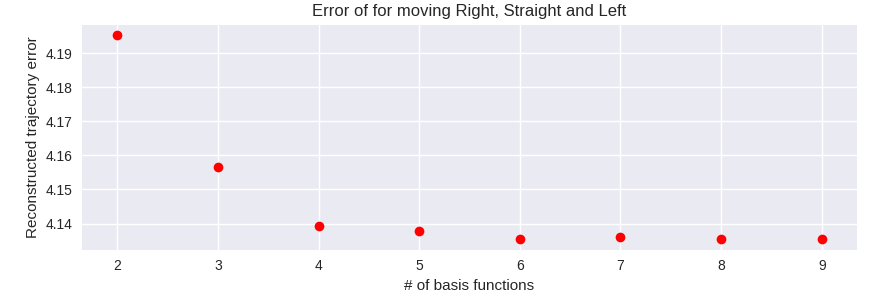
\includegraphics[width=13cm]{img/org_error.png}
	\caption{Error value between original and reconstructed trajectories}
	\label{fig:orgError}    
\end{figure}

As it is possible to see from Figure~\ref{fig:orgError}, having $6$ and more \glspl{RBF} gives the smallest error. Since more \glspl{RBF}, means the longer computation time, from now we will use $6$ and a constant number for \glspl{RBF}, while working with this set of demonstrations. Figure~\ref{fig:primitives}

\begin{figure}[H]
	\centering  	
	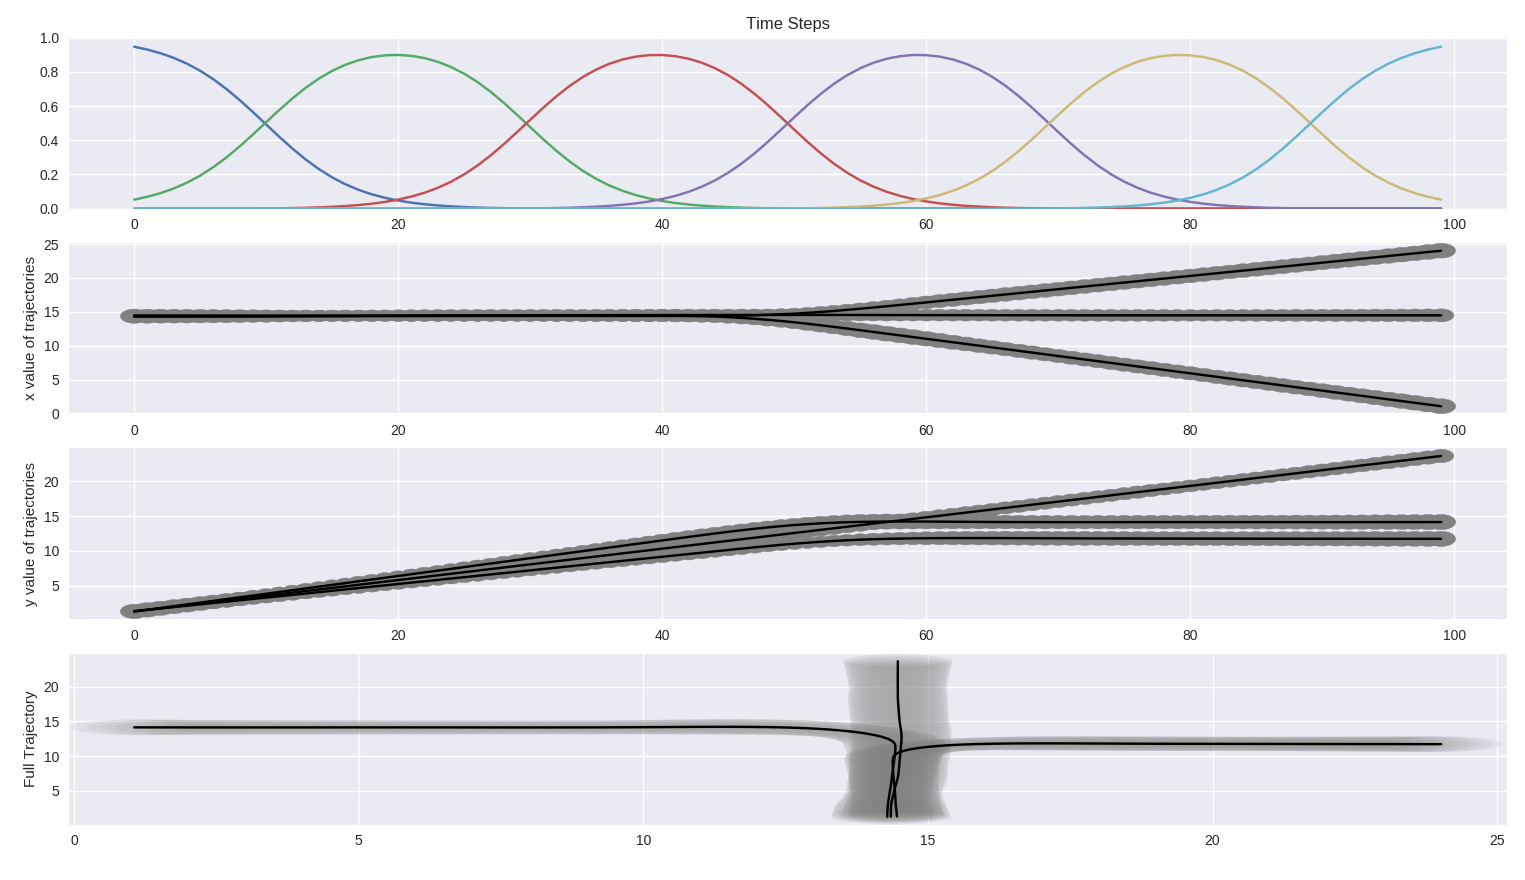
\includegraphics[width=17cm]{img/primitives.png}
	\caption{All primitives from \gls{ProMPs}. The first picture shows how \glspl{RBF} looks like, the second and third pictures shows primitives and demonstrations for x and y dimensions respectively and the last picture shows the full trajectory}
	\label{fig:primitives}    
\end{figure}